\documentclass[12pt,a4paper]{book} % article, report, book.
\input{A1.Preambulo.paquetes.tex}
\input{A2.Preambulo.commandos.tex}
\input{A3.Preambulo.entornos.tex}
\input{A4.Preambulo.estilodepagina.tex}
\usepackage{epstopdf}
\begin{document}

%%%%%%%%%%%%%%%%%%%%%%%%%%%%%%%%%%%%%%%%%%%%%%%%%%%%%%%%%%%%%%

\chapterbegin{Introducción al ensamblador}
\label{chp:IntrEnsam}
\minitoc

{\bf Objetivo}:
En esta sesión vamos a conocer el entorno de trabajo.
Veremos qué aspecto tiene un programa en ensamblador, veremos cómo
funcionan los tres programas que vamos a utilizar: el ensamblador,
el {\it enlazador (linker)} y el {\it depurador (debugger)}.
Del {\it debugger} sólo mostraremos unos pocos comandos,
que ampliaremos en las próximas sesiones.
También veremos la representación de los números naturales y de los
enteros, y el funcionamiento de algunas de las instrucciones del ARM.
Se repasarán también los conceptos de registros, flags e instrucciones
para la manipulación de bits.

\section{Lectura previa}

\subsection{Características generales de la arquitectura ARM}

ARM es una arquitectura RISC (Reduced Instruction Set Computer=Ordenador
con Conjunto Reducido de Instrucciones) de 32 bits, salvo la versión del
core ARMv8-A que es mixta 32/64 bits (bus de 32 bits con registros de 64
bits). Se trata de una arquitectura licenciable, quiere decir que la
empresa desarrolladora ARM Holdings diseña la arquitectura, pero son
otras compañías las que fabrican y venden los chips, llevándose ARM
Holdings un pequeño porcentaje por la licencia.

%\begin{figure}[h]
%  \centering
%    \includegraphics[width=13cm]{graphs/ArmRoadMap.jpg}
%  \caption{Clasificación de Familias ARM}
%  \label{fig:clasif_fami}
%\end{figure}

El chip en concreto que lleva la Raspberry Pi es el BCM2835, se trata de
un SoC (System on a Chip=Sistema en un sólo chip) que contiene además de
la CPU otros elementos como un núcleo GPU (hardware acelerado OpenGL
ES/OpenVG/Open EGL/OpenMAX y decodificación H.264 por hardware) y un
núcleo DSP (Digital signal processing=Procesamiento digital de señales)
que es un procesador más pequeño y simple que el principal, pero
especializado en el procesado y representación de señales analógicas.
La CPU en cuestión es la ARM1176JZF-S, un chip de la familia ARM11 que
usa la arquitectura ARMv6k. 

\begin{longtable}{| p{4.2cm} | p{2.5cm} | p{1cm} | p{6cm} |}
\hline
{\bf Familia} & {\bf Arquitectura} & {\bf Bits} & {\bf Ejemplos de dispositivos} \\ \hline
ARM1      & ARMv1       & 32/26 & Segundo procesador BBC Micro \\ \hline
ARM2, ARM3, Amber & ARMv2      & 32/26 & Acorn Archimedes \\ \hline
ARM6, ARM7 & ARMv3      & 32 & Apple Newton Serie 100 \\ \hline
ARM8, StrongARM & ARMv4       & 32 & Apple Newton serie 2x00 \\ \hline
ARM7TDMI,\newline ARM9TDMI & ARMv4T & 32 & Game Boy Advance \\ \hline
ARM7EJ, ARM9E,\newline ARM10E, XScale & ARMv5 & 32 & Samsung Omnia,\newline Blackberry 8700 \\ \hline
ARM11     & ARMv6 & 32 & iPhone 3G, Raspberry Pi \\ \hline
Cortex-M0/M0+/M1 & ARMv6-M & 32 & \\ \hline
Cortex-M3/M4 & ARMv7-M ARMv7E-M & 32 & Texas Instruments Stellaris \\ \hline
Cortex-R4/R5/R7 & ARMv7-R & 32 & Texas Instruments TMS570 \\ \hline
Cortex-A5/A7/A8/A9\newline A12/15/17, Apple A6 & ARMv7-A & 32 & Apple iPad \\ \hline
Cortex-A53/A57, X-Gene, Apple A7 & ARMv8-A & 64/32 & Apple iPhone 5S\\ \hline
\caption{Lista de familias y arquitecturas ARM}
\label{list_fam}
\end{longtable}

Las extensiones de la arquitectura ARMv6k frente a la básica ARMv6 son mínimas
\footnote{\url{http://infocenter.arm.com/help/index.jsp?topic=/com.arm.doc.ddi0301h/apbs02s02.html}}
por lo que a efectos prácticos trabajaremos con la arquitectura ARMv6.

\subsubsection{Registros}
La arquitectura ARMv6 presenta un conjunto de 17 registros (16 principales
más uno de estado) de 32 bits cada uno.
\newline

\begin{figure}[h]
  \centering
    \includegraphics[width=14cm]{graphs/registros.png}
  \caption{Registros de la arquitectura ARM}
  \label{fig:reg_arm}
\end{figure}

\begin{descript}
  \item[Registros Generales.]
    Su función es el almacenamiento temporal de datos. Son los 13 registros
    que van R0 hasta R12.
  \item[Registros Especiales.]
    Son los últimos 3 registros principales: R13, R14 y R15. Como son de
    propósito especial, tienen nombres alternativos.

    \begin{itemize}
      \item{\textbf{SP}/R13. Stack Pointer ó Puntero de Pila. Sirve como puntero para almacenar
        variables locales y registros en llamadas a funciones.}
      \item{\textbf{LR}/R14. Link Register ó Registro de Enlace. Almacena la dirección de retorno
        cuando una instrucción BL ó BLX ejecuta una llamada a una rutina.}
      \item{\textbf{PC}/R15. Program Counter ó Contador de Programa. Es un registro que indica
        la posición donde está el procesador en su secuencia de instrucciones. Se
        incrementa de 4 en 4 cada vez que se ejecuta una instrucción, salvo que ésta
        provoque un salto.}
    \end{itemize}

  \item[Registro CPSR.]
        Almacena las banderas condicionales y los bits de control. Los bits de control
        definen la habilitación de interrupciones normales (I),
        interrupciones rápidas (F), modo Thumb \footnote{es un modo simplificado donde las
        instrucciones son de 16 bits en lugar de 32 y se acceden a menos registros (hasta r7),
        con la ventaja de que el código ocupa menos espacio.} (T) y el modo de operación
        de la CPU. Existen hasta 8 modos de operación, pero desde nuestra aplicación
        sólo vamos a trabajar en uno de ellos, el {\it Modo Usuario}. Los demás son modos
        privilegiados usados exclusivamente por el sistema operativo.

        Desde el {\it Modo Usuario} sólo podemos acceder a las banderas condicionales, que
        contienen información sobre el estado de la última operación realizada por la ALU.
        A diferencia de otras arquitecturas en ARMv6 podemos elegir si queremos que una
        instrucción actualice o no las banderas condicionales, poniendo una "s" detrás
        del nemotécnico \footnote{Es la forma de nombrar las instrucciones desde
        ensamblador, normalmente derivadas de una abreviatura del verbo en inglés. Por
        ejemplo la instrucción {\it MOV} viene de "move" (mover) }. Existen 4 banderas
        y son las siguientes:

    \begin{itemize}
      \item{\textbf{N}. Se activa cuando el resultado es negativo.}
      \item{\textbf{Z}. Se activa cuando el resultado es cero o una comparación es cierta.}
      \item{\textbf{C}. Indica acarreo en las operaciones aritméticas.}
      \item{\textbf{V}. Desbordamiento aritmético.}
    \end{itemize}
\end{descript}


\subsubsection{Esquema de almacenamiento}

El procesador es {\it Bi-Endian}, quiere decir que es configurable entre {\it Big Endian}
y {\it Little Endian}. Aunque nuestro sistema operativo nos lo limita a {\it Little Endian}.

Por tanto la regla que sigue es "el byte menos significativo ocupa la posición más baja".
Cuando escribimos un dato en una posición de memoria, dependiendo de si es byte, half word
o word,... se ubica en memoria según el esquema de la figura 1.1. La dirección de un dato
es la de su byte menos significativo. La memoria siempre se referencia a nivel de byte, es
decir si decimos la posición N nos estamos refiriendo al byte N-ésimo, aunque se escriba
media palabra, una palabra,...

***cambiar los textos del .pdf por strb r1, [r0]  strh r1, [r0]  str  r1, [r0]  
\begin{figure}[h]
  \centering
    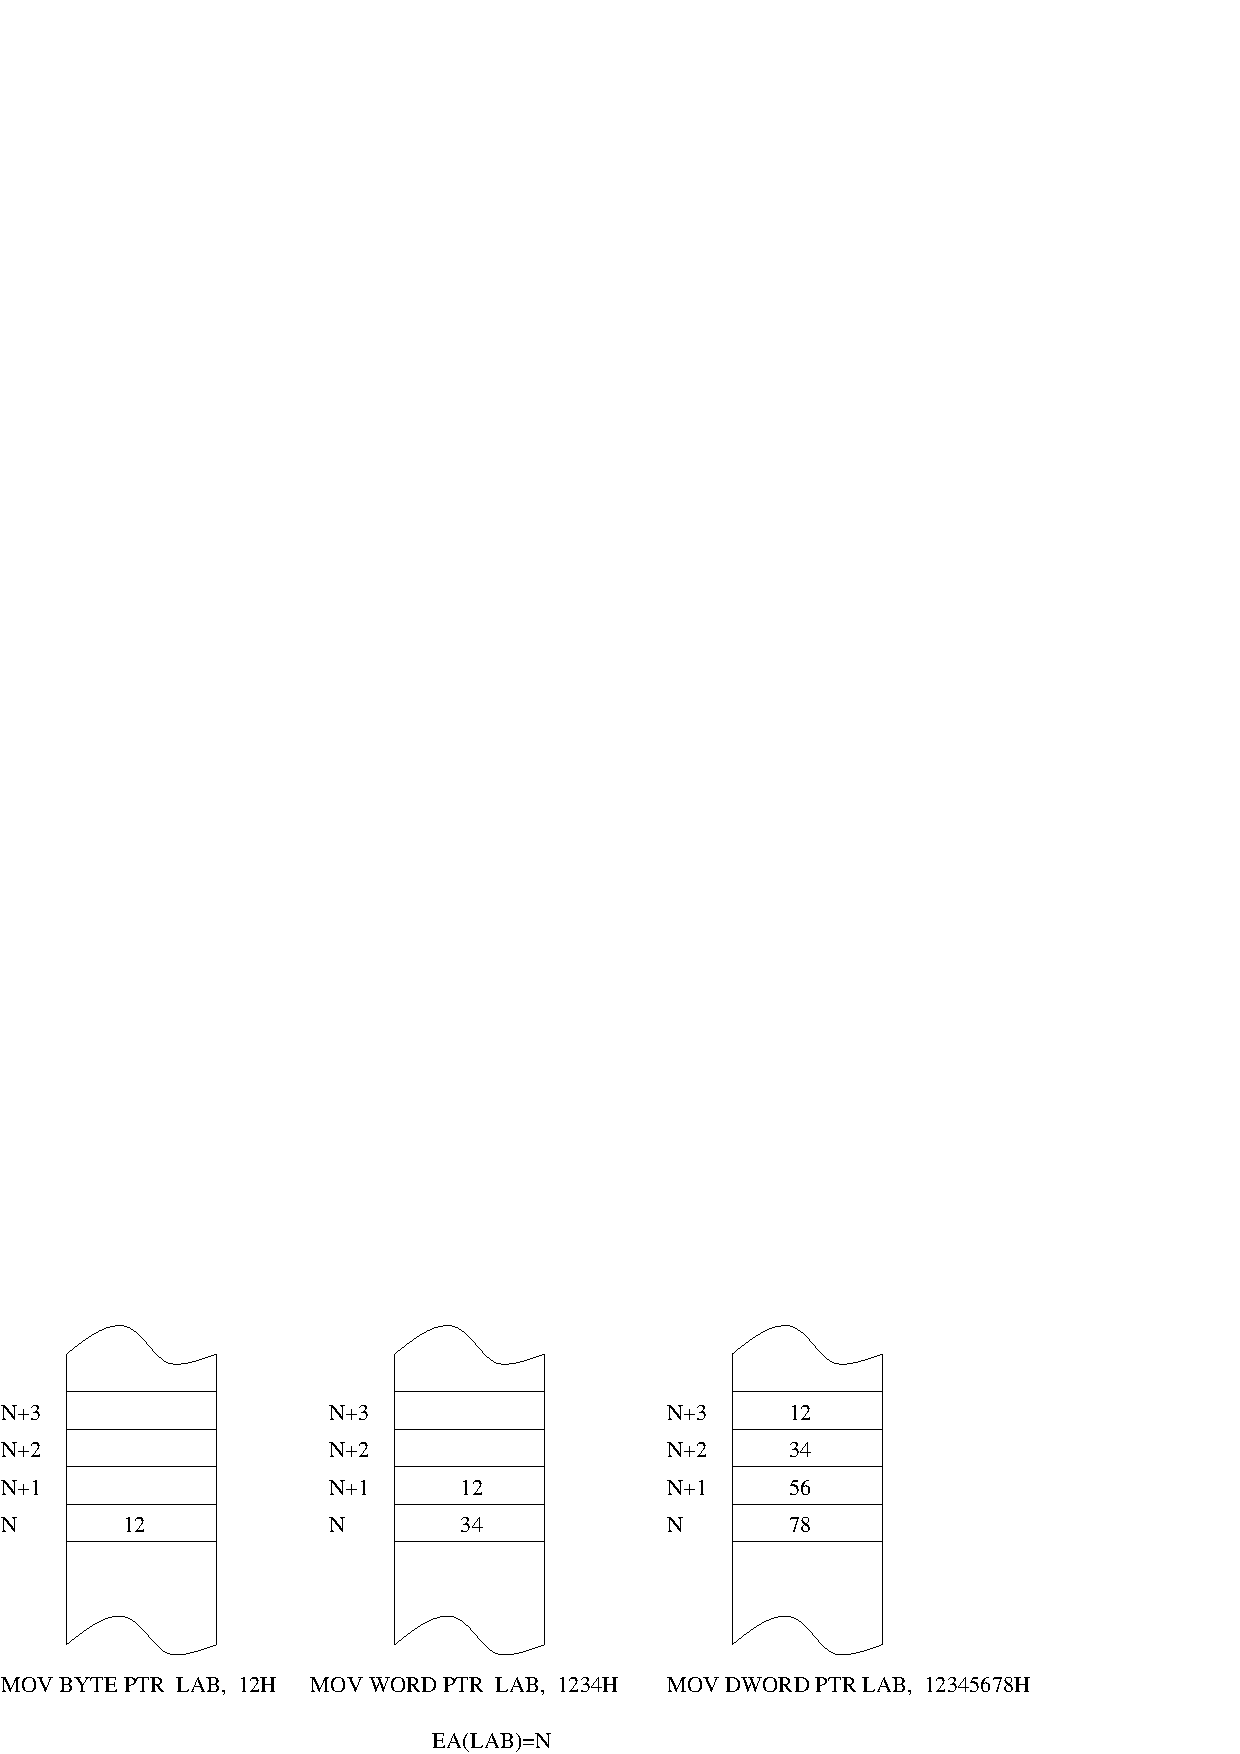
\includegraphics[width=13cm]{graphs/memo.pdf}
  \caption{Ubicación de datos en memoria}
  \label{fig:memo}
\end{figure}

\subsection{El lenguaje ensamblador}

El ensamblador es un lenguaje de bajo nivel que permite un control
directo de la CPU y todos los elementos asociados. Cada línea de un
programa ensamblador consta de una instrucción del procesador y la
posición que ocupan los datos de esa instrucción.

Desarrollar programas en lenguaje ensamblador es un proceso laborioso.
El procedimiento es similar al de cualquier lenguaje compilado.
Un conjunto de instrucciones y/o datos forman un módulo fuente.
Este módulo es la entrada del compilador, que chequea la sintaxis y lo
traduce a código máquina formando un módulo objeto.
Finalmente, un enlazador (montador ó {\it linker}) traduce todas las
referencias relativas a direcciones absolutas.

El ensamblador presenta una serie de ventajas e inconvenientes con
respecto a otros lenguajes de más alto nivel. Al ser un lenguaje de
bajo nivel, presenta como principal característica la flexibilidad y
la posibilidad de acceso directo a nivel de registro. En
contrapartida, programar en ensamblador es laborioso puesto que los
programas contienen un número elevado de líneas y la corrección y
depuración de éstos se hace difícil.

Generalmente, y dado que crear programas un poco extensos es
laborioso, el ensamblador se utiliza como apoyo a otros lenguajes
de alto nivel para 3 tipos de situaciones:
\begin{itemize}
     \item[-] Operaciones que se repitan un número elevado de veces.
     \item[-] Cuando se requiera una gran velocidad de proceso.
     \item[-] Para utilización y aprovechamiento de dispositivos y
     recursos del sistema.
\end{itemize}

\subsection{El entorno}

Los pasos habituales para hacer un programa (en cualquier lenguaje) son 
los siguientes:
lo primero es escribir el programa en el lenguaje fuente
mediante un editor de programas.
El resultado es un fichero en un lenguaje que puede entender el usuario,
pero no la máquina.
Para traducirlo a lenguaje máquina hay que utilizar un programa traductor.
Éste genera un fichero con la traducción de dicho programa, pero todavía
no es un programa ejecutable.
Un fichero ejecutable contiene el programa traducido más una serie de
códigos que debe tener todo programa que vaya a ser ejecutado en una
máquina determinada.
Entre estos códigos comunes se encuentran las librerías del lenguaje.
El encargado de unir el código del programa con el código de estas
librerías es un programa llamado montador ({\it linker}) que genera el
programa ejecutable (ver la figura \ref{fig:entorno})

***cambiar los .asm por .s
\begin{figure}[h]
  \centering
    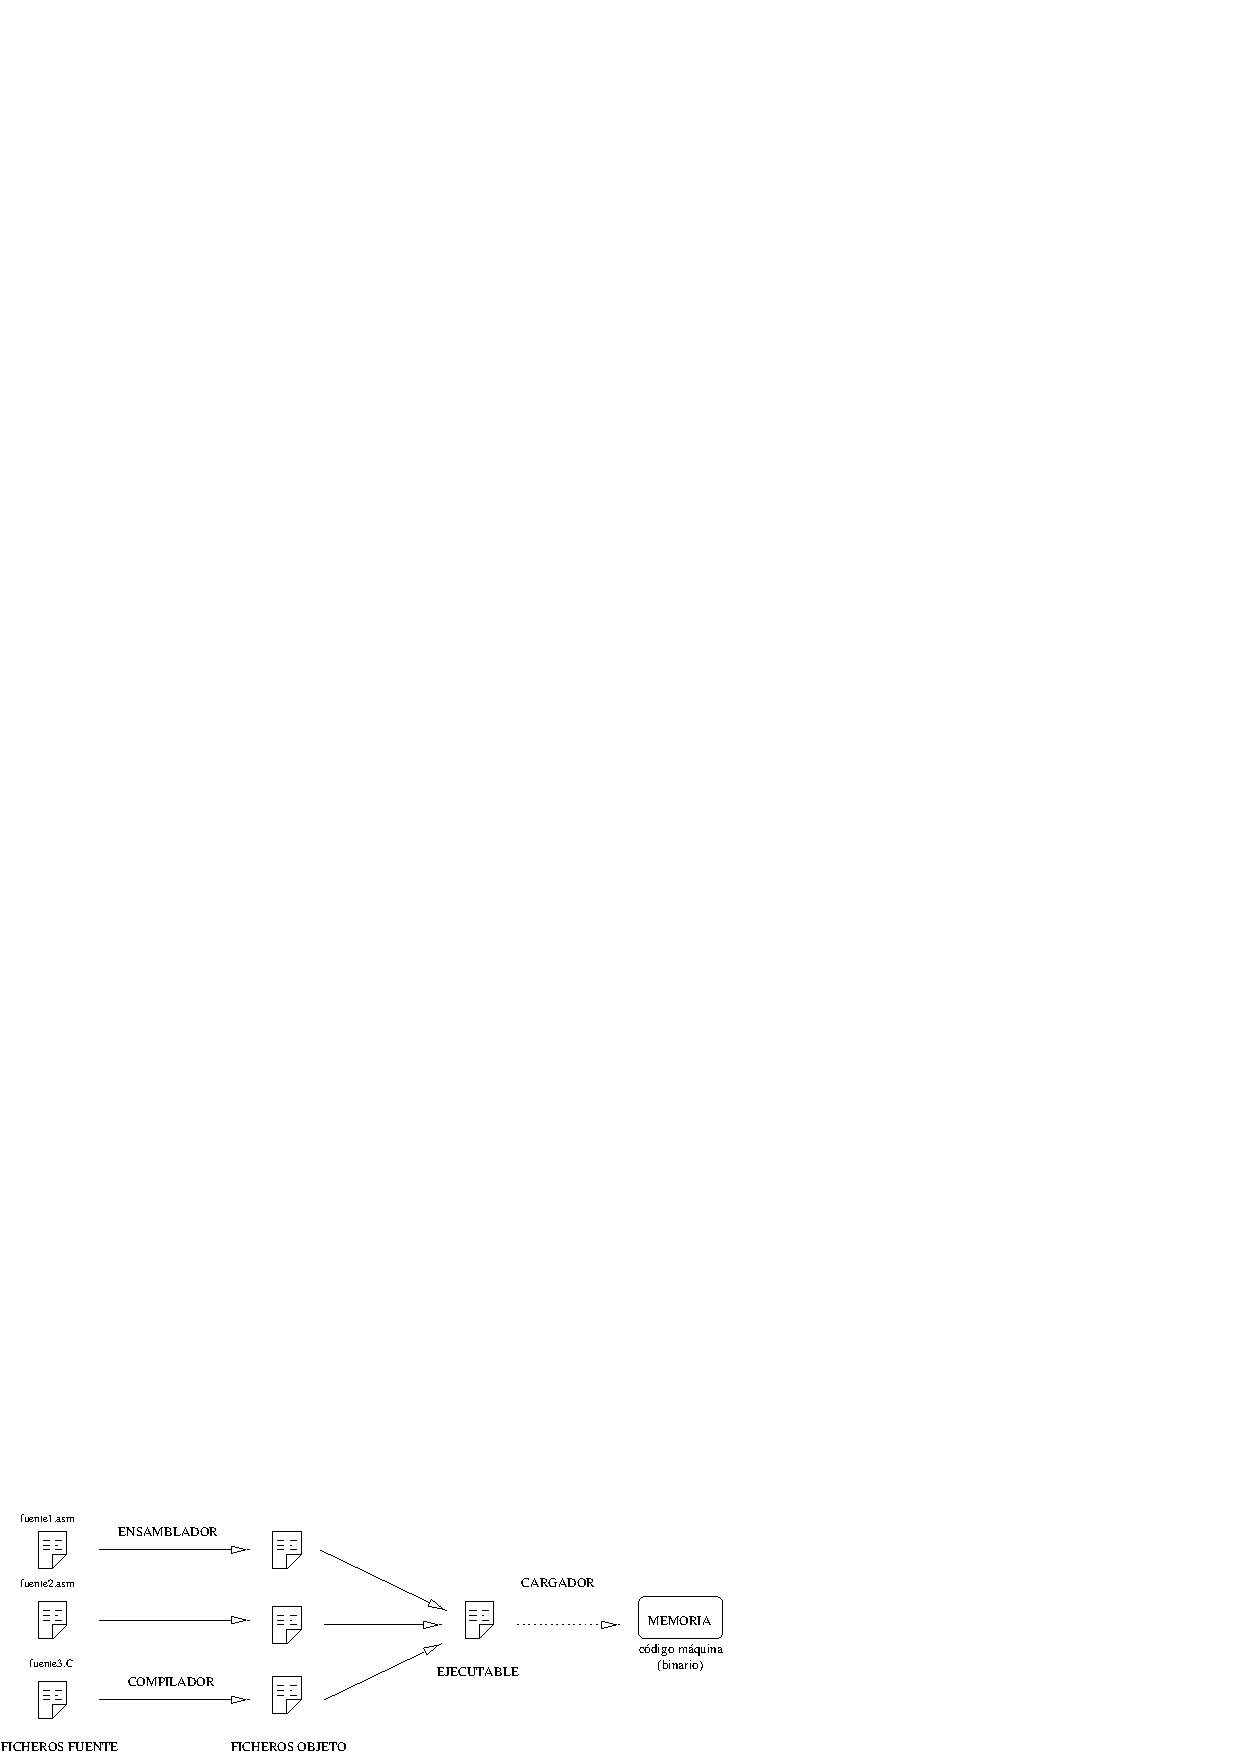
\includegraphics[width=13cm]{graphs/ensamblado.pdf}
  \caption{Entorno típico de programación}
  \label{fig:entorno}
\end{figure}

Durante el proceso de creación de un programa se suelen producir errores.
Hay dos tipos de errores: los sintácticos o detectables en tiempo de
traducción y los errores semánticos o detectables en tiempo de ejecución.
Los errores sintácticos son, por ejemplo, escribir mal una instrucción o
hacer una operación entre dos tipos de datos incompatibles.
Estos errores son detectados por el traductor y se deben solucionar para
poder generar un ejecutable.

Una vez que se tiene un programa sintácticamente correcto lo podemos
ejecutar, pero ésto no implica que el programa sea correcto. Todas las
instrucciones pueden ser correctas, pero se puede haber olvidado poner la
condición de salida de un bucle (y que no termine nunca) o que
sencillamente el programa no haga lo que queremos.

Estos errores sólo se pueden detectar en tiempo de ejecución.
Para poder eliminarlos se utiliza un depurador de programas ({\it debugger}).
El depurador nos permite ejecutar el programa instrucción a instrucción y
ver todos los valores que se van a calcular, de manera que podemos encontrar
los errores.

En el laboratorio utilizaremos el editor {\bf nano} para crear
y editar los módulos fuente de nuestros programas. El traductor
(que en el caso de traducir de un lenguaje ensamblador a lenguaje máquina
recibe el nombre de ensamblador), el {\it linker} y el {\it debugger} son
respectivamente GNU Assembler ({\bf AS}), GNU Compiler Collection ({\bf GCC})
y GNU Debbuger ({\bf GDB}). Todas estas herramientas forman parte de la
GNU toolchain que viene instalada por defecto en la mayoría de las distribuciones
basadas en Linux, en concreto Raspbian. Para obtener más información sobre estos
comandos se puede recurrir a la ayuda del sistema con <man as>, <man gcc> y
<man gdb>. Se aconseja que a lo largo de de esta
primera sesión práctica os vayais familiarizando con ambos entornos,
aunque no se os indique explícitamente.

\subsection{Aspecto de un programa en ensamblador}

En el listado \ref{lst:codigoPract1} se muestra el código de la primera
práctica que probaremos. En el código hay una serie de elementos que
aparecerán en todos los programas y que estudiaremos a continuación.

La principal característica de un módulo fuente en ensamblador es
que existe una clara separación entre las instrucciones y los
datos. De hecho, un módulo fuente puede estar formado por tres bloques
independientes que se van a ubicar en tres segmentos distintos en la
memoria RAM.

\begin{lstlisting}[caption={Código del programa intro1.s},label={lst:codigoPract1},numbers=left,escapeinside={@}{@}]
.data

var1:   .word   3
var2:   .word   4
var3:   .word   0x1234

.text
.global main
.func main
 
main:   ldr     r1, puntero_var1    /* r1 <- &var1    */
        ldr     r1, [r1]            /* r1 <- *r1      */
        ldr     r2, puntero_var2    /* r2 <- &var2    */
        ldr     r2, [r2]            /* r2 <- *r2      */
        ldr     r3, puntero_var3    /* r3 <- &var3    */
        add     r0, r1, r2          /* r0 <- r1 + r2  */
        str     r0, [r3]            /* *r3 <- r0      */
        bx      lr

puntero_var1:   .word   var1
puntero_var2:   .word   var2
puntero_var3:   .word   var3
\end{lstlisting}


\chapterend{}

%%%%%%%%%%%%%%%%%%%%%%%%%%%%%%%%%%%%%%%%%%%%%%%%%%%%%%%%%%%%%%
\end{document}